\documentclass[12pt, twoside]{article}
\usepackage[letterpaper, margin=1in, headsep=0.5in]{geometry}
\usepackage[english]{babel}
\usepackage[utf8]{inputenc}
\usepackage{amsmath}
\usepackage{amsfonts}
\usepackage{amssymb}
\usepackage{tikz}
\usepackage{yhmath}
%\usetikzlibrary{quotes, angles}

\usepackage{graphicx}
\usepackage{enumitem}
\usepackage{multicol}

\usepackage{fancyhdr}
\pagestyle{fancy}
\fancyhf{}
\renewcommand{\headrulewidth}{0pt} % disable the underline of the header

\fancyhead[RE]{\thepage}
\fancyhead[RO]{\thepage \\ Name: \hspace{3cm}}
\fancyhead[L]{BECA / Dr. Huson / 10th Grade Geometry\\* 14 May 2019}

\begin{document}
\subsubsection*{11.2 Homework: Density \& trigonometry situations}
 \begin{enumerate}

   \item $\triangle ABC$ is shown with $m\angle C=90^\circ$ and the lengths of the triangle's sides are $BC=6$, $AC=8$, and $AB=10$.
   \begin{multicols}{2}
         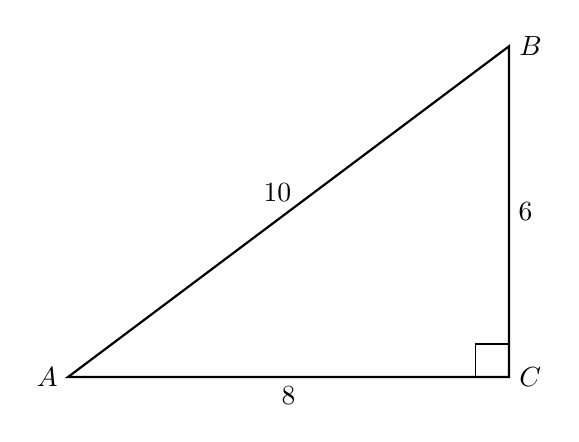
\begin{tikzpicture}[scale=0.7]
           \draw [thick]
           (0,0)node[left]{$A$}--
           (8,0)node[ right]{$C$}--
           (8,6)node[right]{$B$}--cycle;
           \draw (8,0)++(-0.6,0)--++(0,0.6)--+(0.6,0);
           \node at (4,0)[below]{$8$};
           \node at (8,3)[right]{$6$};
           \node at (3.8,3)[above]{$10$};
         \end{tikzpicture}
         \begin{enumerate}
         \item State, as a decimal, the value of $\sin B$. \vspace{1.25cm}
         \item Find the measure of $\angle B$, to the \emph{nearest degree}. \vspace{1.25cm}
         \item Find the degree measure of $\angle A$.
       \end{enumerate}
     \end{multicols}
     \vspace{1.5cm}


   \item Express each trigonometric ratio to the \emph{nearest thousandth} and each angle measure to the \emph{nearest degree}.
     \begin{multicols}{2}
       \begin{enumerate}
         \item $\sin 38^\circ =$ \vspace{0.5cm}
         \item $\cos^{-1} 0.866 =$ \vspace{0.5cm}
       \end{enumerate}
     \end{multicols} \vspace{0.5cm}

   \item Bob places an 18-foot ladder 6 feet from the base of his house and leans it up against the side of his house. Find, to the nearest degree, the measure of the angle the bottom of the ladder makes with the ground. \vspace{5cm}



\end{enumerate}
\end{document}
